To support the key-value cache, each node must implement some form of indexing
service. Each indexing service must support a number of tasks such as
\emph{insertion}, \emph{deletion}, \emph{retrieval}, \emph{eviction} and
\emph{migration}. We consider three distinct but common indexing schemes:
\bptrees\cite{btree,bplustree}, Extendible Hashing\cite{ullman}, and
Counting Bloom Filters\cite{countingbloom1,countingbloom2}.

In order to operate in the elastic environment of our cache, when a node
overflows it must be capable of migrating a subset of its data records to
another node either preexisting or freshly allocated. Each of these schemes
have inherent differences in their structure and operation and, as such, are
compelling candidates for extension into the elastic makeup of \emph{Auspice}.

The remainder of this chapter will present background on each of the indexing
structures, describe the implementation of their migration mechanisms, and
provide an experimental analysis of their performance benchmarks.

\section{\bptrees} % (fold)
\label{sec:b_trees}
B-Trees and \bptrees are used in many of today's systems. The \bptree is a
multilevel indexing scheme that automatically adjusts the number of levels
depending upon the file size and stores all of its records in the leaf nodes.
Each record is stored in ascending order from left to right and each leaf node
is linked to the next and previous nodes. In this way, its design is
specifically crafted to accelerate queries over a range of
values\cite{navathe,ullman}. In terms of retrieval, \bptrees are balanced data
structures, where all paths from the root to any leaf have the same length
(similar to binary trees, with approximately log$_2 n$ depth).

\begin{figure}
\begin{center}
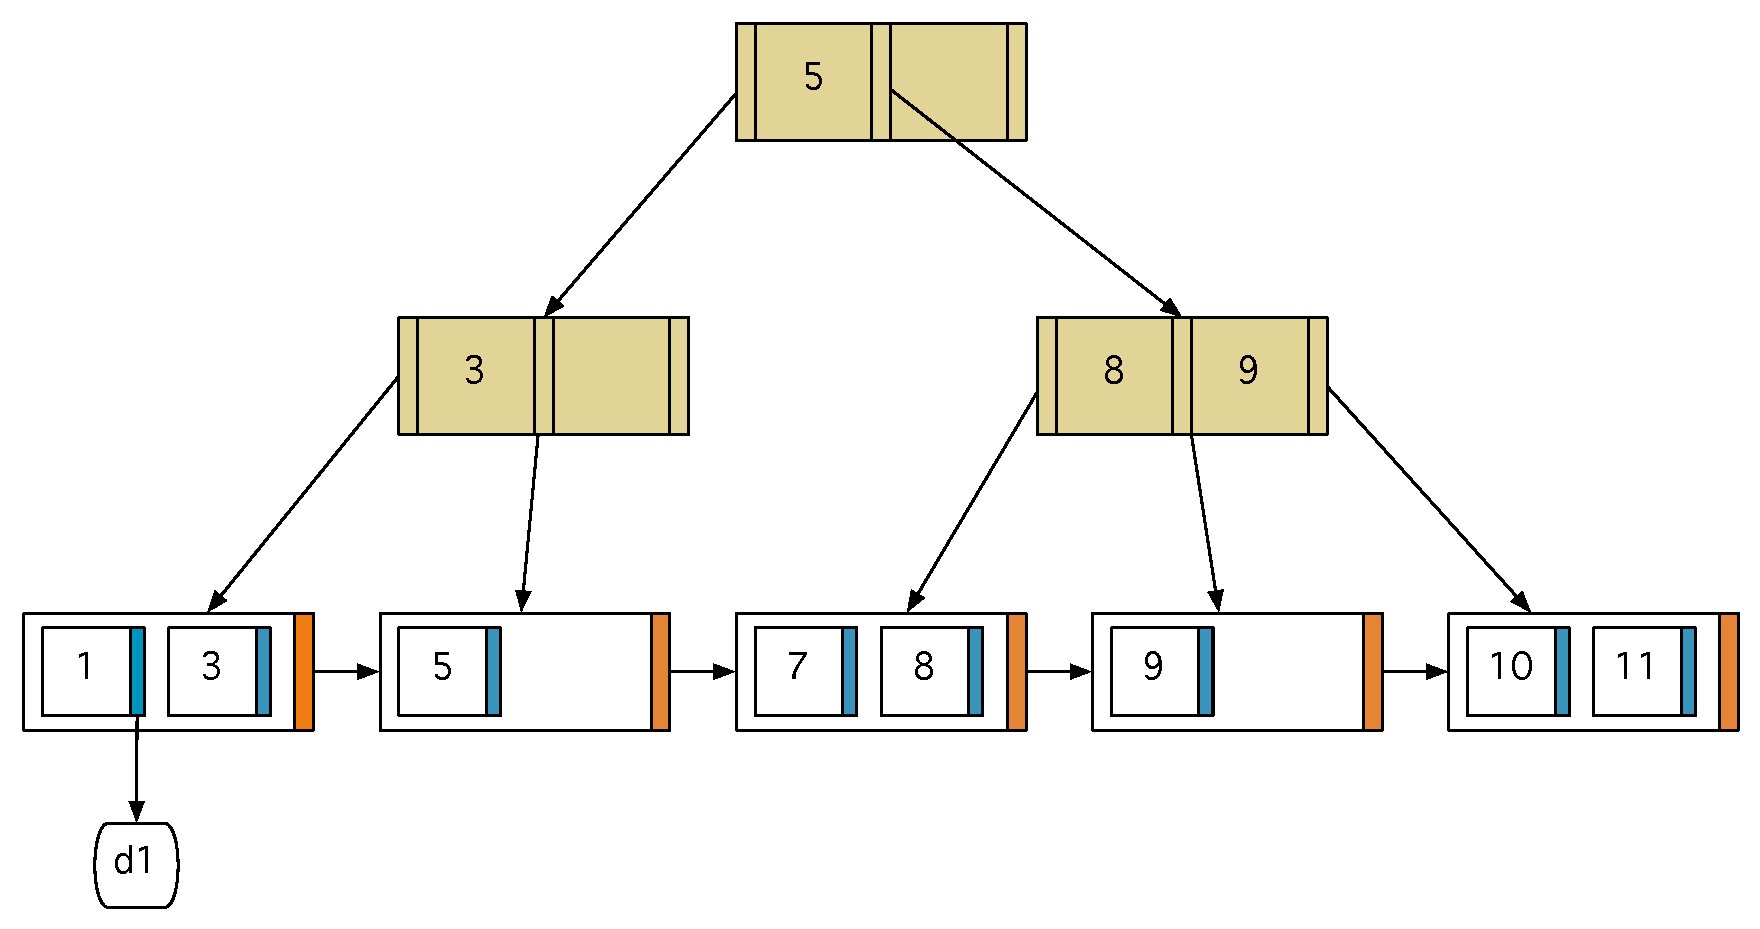
\includegraphics[scale=0.5]{figures/bplustree.pdf}
\end{center}
\caption{\bptree structure}
\label{fig:bplustree}
\end{figure}

Structurally, \bptrees are composed as shown in Figure~\ref{fig:bplustree}.
Internal nodes, those colored beige, act as pointers to other nodes in the
structure. All keys in the left branch of the key \emph{K} are less than or
equal to \emph{K}, while all keys to the right are greater than \emph{K}. While
searching, we compare the search key with the entries in the tree until such a
point as we reach the leaf node. Leaf nodes, those colored white, contain the
stored keys and pointers to the physical data location (blue). Additionally, in
order to assist with range queries, leaf nodes also contain a pointer to the
next leaf node, in order (orange).

With this sort of structure, we can see that range queries are made quite
simple and quick. Given a range $[k_{start}, k_{end}]$ we begin by searching to
find $k_{start}$ then proceed to iterate through the leaves until we find a
node greater than $k_{end}$. The search then returns the set of data identified
in that range. Due to this support, we expect the \bptree integration to be
well suited to elastic cache. Quick access to ranges of data should lead to
much faster data migration in the event of node additions. Data migration,
which is composed of a set of key deletions, can again be efficiently managed
in the same way as a range query is. The \bptree migration algorithm is shown
in Algorithm~\ref{alg:migrate1}.

\begin{algorithm}[htp]
\small
\caption{\label{alg:migrate1}BT\_Migrate($k_{start}$, $k_{end}$)} \begin{algorithmic}[1]
\STATE $\triangleright$ manipulate B$^+$-tree index and transfer the keys in form of a string, $keys$
\STATE $end \leftarrow false$
\STATE $\triangleright$ $L =$ leaf initially containing $k_{start}$ 
\STATE $L \leftarrow btree$.search($k_{start}$)
\WHILE{$(\neg end \wedge L \neq NULL)$}
 \STATE $\triangleright$ each leaf node contains multiple keys
 \FORALL {$(k,v) \in L$}
   \IF {$k \le k_{end}$}
     \STATE $keys$.append($k$, $v$)
     \STATE $btree$.delete($k$)
   \ELSE
     \STATE $end \leftarrow true$
     \STATE break
   \ENDIF
 \ENDFOR
 \STATE $L \leftarrow L$.next()
\ENDWHILE
\STATE return $keys$
\end{algorithmic}
\end{algorithm}

% TODO: This section is cribbed heavily from IJNGC paper, look at rewrite.

% section B_Trees (end)

\section{Extendible Hashing} % (fold)
\label{sec:extendible_hashing}
Hash tables are another ubiquitous form of indexing and are often a favorite
tool of developers looking for key-value storage. These structures excel at
offering constant-time searches, unlike the logarithmic searches of \bptrees.
However, there is a tradeoff in that hash tables are not well-equipped to
handle range queries.

In most hash implementations, we assume there is some hash function $h(k)
\exists [0, B-1]$, where $B$ is the total number of buckets stored in the
table. Each bucket then contains a set of records, stored either in memory or
in secondary storage. Ideally, a hash function maps each key to a distinct
bucket. In practice however, this is seldom possible as the key range is
significantly larger than $B$. Therefore, the buckets typically allow for the
storage of a set of records. Even still, they can overflow. To avoid this, hash
tables implement some form of collision resolution. One of the most simple
techniques is to have the bucket overflow into a chain. Records mapping to an
already occupied bucket are stored in a linked list format attached to that
bucket. This performance of this solution degrades linearly as the number of
records $K$, and more importantly, the ratio of $K$ to $B$ increases.

We can avoid this problem by using dynamic hashing\cite{dh2}, where the number
of buckets, $B$, is variable. In dynamic hashing schemes, $B$ is increased whenever
necessary. For the purposes of our elastic cache, we have implemented a form of
dynamic hashing called Extendible Hashing\cite{dh1}, which introduces the
concept of a \emph{directory} -- an array of pointers to the hash buckets. The
buckets then contain an additional array of pointers to the physical location
of the records.

Initially, each directory contains a single bucket and is allowed to grow
when required. In Extendible Hashing, the length of the directory is always a
power of two, which means that each growing phase doubles the size of the
directory. Because multiple pointers can reference the same physical bucket,
the number of actual buckets can be less than or equal to the size of the
directory. A hash function $h(k)$ computes a binary sequence for each record
based on the search key, $k$, and the first $i$ least significant bits are used
to determine the bucket to which the record belongs. When a directory contains
$2^i$ pointers to buckets, the actual number of buckets is $\leq 2^i$.

Searching for a key in an extendible hash table is done in two steps. First,
the hash function is run over the key, and the least significant $i$ bits are
used to determine the bucket the key belongs to. Once the bucket has been
identified, a linear scan is run over the contents of the bucket to return the
position of the record, if found. Again, the search time increases as the
number of records per bucket increases. A large number of records per bucket is
also indicative of fewer splits and a smaller directory. As the directory size
increases, the number of records per bucket should thin out in the general
case. As mentioned earlier, while Extendible Hashing offers $O(1)$ time
exact-match queries, range queries suffer as the hash function disrupts $k$'s
original locality.

To support migration, we implemented Extendible Hashing in such a way that we
could dynamically specify the number of records per bucket. Because Extendible
Hash tables do not store the records in a particular order, we must linearly
scan through each bucket and delete keys that lie within the migration range.

The migration procedure takes as input, the range of keys to be migrated,
$[k_{start}, k_{end}]$. We begin by traversing all directories, and for each
directory we follow the pointer to its corresponding bucket. Any key, $k$, which
lies in the migration range is appended, along with its data object, to an
array. This array is returned once all records have been scanned. This
process is shown in Algorithm~\ref{alg:migrate2}.

\begin{algorithm}[htp]
\small
\caption{\label{alg:migrate2}EH\_Migrate($k_{start}$, $k_{end}$)} \begin{algorithmic}[1]
\STATE static $H$ $\triangleright$ bring extendible hashtable to scope
\STATE $keys \leftarrow \{\}$
\FOR {$x \leftarrow 0$ to  $2^i-1$}
  \STATE $D_x \leftarrow H$.getDirectoryAt($x$)
 \FOR {$y \leftarrow 0$ to $|D_x|-1$}
   \STATE $B_y \leftarrow D_x$.getBucketAt($y$)
   \FORALL {$k \in B_y | k \ge k_{start} \wedge k \le k_{end}$}
       \STATE $keys \leftarrow keys \cup~(k,v)$
       \STATE $H$.delete($k$)
   \ENDFOR
 \ENDFOR
\ENDFOR
\STATE return $keys$
\end{algorithmic}
\end{algorithm}

% section extendible_hashing (end)

\section{Bloom Filters} % (fold)
\label{sec:bloom_filters}

Bloom Filters\cite{bloomfilter1} are probabilistic data structures used to
quickly determine the membership of a record in a set. It is composed of a
$m$-bit length bit array and a set of $j$ hash functions, each of which hashes
a set element to one of the $m$ different values. Generally, $m \gg j$, which
reduces the probability of the hash function setting the same bit for a record.
Though Bloom Filters are vulnerable to false positives, false negatives are not
possible.

Insertions into a Bloom Filter are simple: apply the hash function to the key
and set the corresponding bits. Determining membership is also simple: apply
each of the $j$ hash functions to the key and verify if the corresponding bits
are set. If any of the $j$ bits are not set, then the element is not present.
However, because false positives are possible, even if each of the bits are
set, the record may still not be present, and so a scan becomes necessary after
a pseudo-hit. Fortunately, the false positive rate has a bound $f = (1 -
e^{(-jN/m)})^j$, where $j$ is the number of hash functions, $m$ is the length
of the bit array, and $N$ is the number of set bits. From this, we can clearly
see that the false positive rate increases as the number of inserts increases.
By choosing a relatively large $m$ and independent hash functions, we can
render the false positive rate negligible\cite{falsepositive}.

Traditionally, Bloom Filters disallow deletions as the same bit can be set for
multiple records. By modifying the bit array, false negatives would become a
possibility, which are prohibitive. To support deletion, we implemented a
variant called Counting Bloom Filters\cite{countingbloom1,countingbloom2}. Each
bit in the bit array is associated with a 4-bit counter, which then keeps track
of the number of records that set the bit. This counter enables the delete
operation.

These structures are most useful for applications that require fast tests of
record existence, and especially beneficial for those that test non-existence.
To search for a record with key $k$, we apply the $j$ hash functions to $k$. We
then $AND$ all bits from the bit array corresponding to the locations $h_i(k) |
i = (0,\ldots,j)$. If the result of this operation is one, then the record may be
present and a scan is performed to retrieve the record. If the result is zero,
the record is non-existence. Because a linear scan may be required for a hit,
there is a costly overhead involved in the case of false positives. However, as
mentioned, low false positive rates can be ensured by having a large $m$ and
independent hash functions.

Implementing migration in a Counting Bloom Filter is also quite simple. Again
we operate over the range $[k_{start},k_{end}]$. We begin from the minimum
threshold and increment until we reach the maximum threshold, searching for
each key in the range. Keys that are present are then deleted. This makes
migration time linear to the amount of keys within $[k_{start},k_{end}]$. This
algorithm is demonstrated in Algorithm~\ref{alg:migrate3}.

\begin{algorithm}[htp]
\small
\caption{\label{alg:migrate3}CBF\_Migrate($k_{start}$, $k_{end}$)} \begin{algorithmic}[1]
\STATE static $H$ $\triangleright$ counting bloom filter to scope
\STATE $keys \leftarrow \{\}$
\FOR {$k \leftarrow k_{start}$ to  $k_{end}$}
  \IF {$H$.contains($k$)}
    \STATE $v \leftarrow H$.retrieve($k$)
    \IF {$v \neq$ NULL}
      \STATE $keys \leftarrow keys \cup~(k,v)$
    \ENDIF
  \ENDIF
\ENDFOR
\STATE return $keys$
\end{algorithmic}
\end{algorithm}
% section bloom_filters (end)

\section{Elastic Cache Support} % (fold)
\label{sec:elastic_cache_support}
We have implemented this system on EC2 and here we describe the system within
that context. The Amazon Elastic Compute Cloud (EC2) supports
Infrastructure-as-a-Service (IaaS), allowing users to allocate nodes on demand.
EC2 nodes (\emph{instances}) are virtual machines that can launch system
snapshots (\emph{images}). These virtual machines are deployed onto various
architectures (\emph{instance types}) with varying costs depending upon their
capabilities. As a baseline, we have chosen to use only small instances in our
implementation, though there are instances with far greater (and fewer)
capabilities available.

During system execution, records may continually be inserted into the cache
nodes. Overflow of any individual node may invoke an incremental scaling
effort. This process involves starting a new EC2 node and migrating a subset of
the data from the overflown node to the newly allocated node. There are two
areas of overhead in this process: (1) instance allocation time, which can take
up to several minutes during peak time, and (2) data migration time, which
involves identifying the migration range and network transfer time.

In our experience, instance allocation time dominates that of data migration.
We thus, implement a system that pre-launches instances speculatively when some
threshold, $T$, has been met. At background thread initiates the pre-launching
and begins to eagerly migrate data from the fullest node once the new one has
been booted. Out threshold $T$ is based on the following observations: if the
request rate is high, then $T$ should be lowered, as the nodes are likely to
fill up faster. Conversely, if the request rate is low, then $T$ should be
raised. If $n$ is the node to insert some $(k,v)$ pair, we use the following to
estimate $n$'s threshold.
\begin{center}
  $T = c(n)/2 + \delta_H \times (||N|| - R/\delta_L)$
\end{center}
where $\delta_L$ and $\delta_H$ are constants: the lowest and highest
\emph{expected} querying rate respectively. $R$ is the current request rate,
$c(n)$ is the capacity of node $n$ and $||N||$ is the total number of nodes in
our cache. As the number of nodes, $||N||$ increases, the threshould should
also increase so as to delay the allocation of new nodes. $R/\delta_L$ is used
to normalize the current rate, $R$.

We use this threshold in our cache insertion algorithm, shown in
Algorithm~\ref{alg:optimize}. The identifiers used in
Algorithm~\ref{alg:optimize} are listed in Table~\ref{tab:vars1}.

\begin{table}[htp]
\caption{\label{tab:vars1}Listing of Identifiers for Algorithm~\ref{alg:optimize}}
\centering
\begin{tabular}[]{| c || p{5.5cm} |}
  \hline
  \textbf{Identifier} & \textbf{Description} \\
  \hline
  \hline

  $k$ & A queried key \\
  \hline
  $B = (b_1, \ldots, b_p)$ & The list of all buckets on the hash line\\
  \hline
  $h(k)$ & The hash function, which returns the closest upper bucket to $k$ \\
  \hline
  $N =(n_1, \ldots, n_m)$  & The set of all nodes in the cooperative cache \\
  \hline
  $n \in N$  & A cache node  \\
  \hline
  $||n||$  & Current size of index on node $n$  \\
  \hline
  $\lceil{n}\rceil$  & Overall capacity on node $n$ \\
  \hline
 $||N||$  & Number of nodes part of the cooperative cache $N$  \\
  \hline
  $R$  & Query intensity, i.e.\ queries per time step  \\
\hline
  \end{tabular}
\end{table}

\begin{algorithm}[htp]
\small
\caption{\label{alg:optimize}Speculative-Insert($k$, $v$, $\delta_L$,
$\delta_H$)} \begin{algorithmic}[1] \STATE static $NodeMap[\ldots]$
\STATE static $B = (\ldots)$
\STATE static $h' : K \rightarrow [0,r)$
\STATE $n \leftarrow NodeMap[h'(k)]$
\STATE $T = c(n)/2 + \delta_H \times (||N|| - R/\delta_L)$
\IF {$T < \lceil{n}\rceil \times 0.1$}
	\STATE $T \leftarrow \lceil{n}\rceil \times 0.1 $\ \ \ \ $\triangleright$ to avoid
	extremely low values of threshold
\ENDIF
\IF {$T > (\lceil{n}\rceil \times 0.75) $}
	\STATE $T \leftarrow \lceil{n}\rceil \times 0.95$\ \ \ \ $\triangleright$ to delay
	allocation of new nodes
\ENDIF

\IF {$||n|| + sizeof(v) < T$}
	\STATE $n$.insert($k,v$)\ \ \ \ $\triangleright$ insert directly on node $n$
\ELSIF{$||n|| + sizeof(v) > T$}
	\STATE $\triangleright$ Launch threads $t1,t2$ which would execute the Lines 16 - 22
	\STATE $\triangleright$ find fullest bucket referencing $n$
	\STATE $b_{max} \leftarrow
		\underset{b_i \in B}{\operatorname{argmax}} ||b_i|| \wedge NodeMap[b_i] = n$
	\STATE $k^{\mu} \leftarrow \mu(b_{max})$
	\STATE $n_{dest} \leftarrow n$.migrate($min(b_{max})$, $k^{\mu}$)
	\STATE $\triangleright$ update structures
	\STATE $B \leftarrow (b_1, \ldots, b_i, h'(k^{\mu}), b_{i+1}, \ldots,
	b_p)~|~b_i < h'(k^{\mu}) < b_{i+1}$
	\STATE $NodeMap[h'(k^{\mu}))] \leftarrow n_{dest}$
\ELSE
	\STATE $\triangleright$ $n$ overflows
	\STATE $\triangleright$ Launch Thread $t3$ if $t1$ and $t2$ are not taking care of $n$ and execute Lines 16-22
\ENDIF

\end{algorithmic}
\end{algorithm}

In Algorithm~\ref{alg:optimize}, $k$ and $v$ are the key and value objects
respectively. On lines 1-3, the statically declared inverse hash map,
$NodeMap[\ldots]$, the ordered list of buckets, $B$, and the auxiliary
consistent hash map, $h'$ are brought into scope. $NodeMap[b]$ returns the node
$n$ pointed to by bucket $b$.

Lines 5-11 manage threshold collection. The idle time caused by migration can
be reduced to zero if a good threshold is selected. Managing this, however, is
very tricky: a low value can lead to a higher number of instances being
launched, incurring greater costs for the extra nodes. A higher value threshold
can result in higher idle times as the nodes are being allocated too late. Thus
we can see that threshold selection involves a tradeoff between lowering idle
times and optimizing the number of instances initialized. Line 5 of
Algorithm~\ref{alg:optimize} calculates this threshold value. 

In lines 6-11, we check for two possible conditions. The first condition
increases the threshold to avoid extremely low values, which would cause rapid
expansion for the set of allocated nodes. The second condition increases the
threshold after a certain instant so that there will not be extra, unnecessary
instances being allocated. This helps to reduce cost.

In order to reduce idle times, we need to parallelize the execution of various
parts of the code. Empirically, with our experiments issuing random workloads,
we observed that two instances generally reached capacity at the same time. We
begin by introducing two threads, $t1$ and $t2$, that initialize a new node if
necessary (lines 15-22). If a node reaches capacity, $\lceil{n}\rceil$, then a
third thread, $t3$, will handle the overflown node if neither of the other two
are already handling it (lines 24-25). At any given point, this means there can
be a maximum of four threads running (including the main thread).

Each of the three threads perform the operations on lines 17-22. We begin by
identifying the most full bucket $b_{max}$ referencing $n$. On lines 18-19, we
migrate half of the keys in $b_{max}$ starting from the minimum and moving to
the median, $k^{\mu}$. The migration method returns a reference to the
destination node, $n_{dest}$, which may already exist or be newly allocated.
Finally, $NodeMap$ and $B$ are updated.

On the cache servers, each cooperating node consists of the index,
\emph{insert}, \emph{delete}, \emph{migrate}, and \emph{search} methods. At any
instance of time, the consistency of the index must be maintained, meaning that
the methods that modify the structure must be synchronized. Thus,
\emph{insert}, \emph{migrate}, and \emph{delete} must begin by acquiring a lock
on the cache server, to be released only at the operation's completion. As
\emph{search} is read-only, this method need not acquire any lock.

% section elastic_cache_support (end)

\section{Hybrid System} % (fold)
\label{sec:hybrid_system}
Finally, for cost effectiveness, we believe it useful to create a hybrid cache.
In this variation, we use only \emph{one} EC2 node and evict records into S3 in
contrast to the other versions, which grow incrementally without eviction. We
believe this configuration offers an effective means of storing the same
quantity of keys, at the slight performance cost of having to query S3. The key
search function initially queries the EC2 node, and upon a miss, searches in
S3.

% section hybrid_system (end)

\section{Experiments} % (fold)
\label{sec:experiments_indexing}
In all experiments, we used \emph{small EC2 instances} from the Amazon Cloud
consisting of 1.7 GB of memory, 1 virtual EC2 core -- equivalent to a 1.0-1.2
GHz 2007 Opteron or 2007 Xeon Processor -- on a 32 bit pltform. Each instance
was loaded with an Ubuntu Linux image and a cache server, which contains the
indexing logic.

We ran a real service application, \emph{Shoreline Extraction}, a geodetic web
service. Given the location, $L$, and the time of interest, $T$, the service
retrieves a data file representing the terrain at location $L$, then
interpolates this file with a water level reading, measured at time $T$.
Naturally, the size of the terrain files impacts the execution of this service.
Because we are only interested in measuring the cache's performance we
normalized the data sets such that the execution times are also normalized
(approximately 23 seconds). The service output is small, \eg, $< 1$Kb,
because only a set of points representing the extracted shoreline are returned.

The queries are submitted to the coordinator node and it tries to locate the
results in the cache based on the inputs from the query. If the result is
present in the cache, \ie, it is precomputed via some previous request, it is
retrieved and returned directly to the caller. In case of a miss, the shoreline
extraction service is invoked. The queries are submitted randomly over 64,000
distinct possibilities for each service request. Because we know the key range
in advance, we have also set $r$, the consistent hashing modulo function, to
64,000.

We tested our system under varying query rates. We varied the rates between 50
and 255 queries per time step.  In order to show the cache's elastic behavior,
we submitted $R$ queries per time step. Each time step is a logical iteration
and does not reflect real time. It is worth noting that the granularity of a
time step, whether seconds, minutes, or hours, does not affect the hit/miss
rates of the cache. At each time step, we recorded the average service
execution time (in number of seconds real time), the number of times a query
reuses a cached record (hits), and the number of cache misses.

% section experiments_indexing (end)

\section{Results} % (fold)
\label{sec:results_indexing}

\subsection{Evaluation of Elastic Cache vs. Static Cache} % (fold)
\label{sub:evaluation_elastic_static}
We compared our cooperative elastic cache ({\tt co-op}) against static versions
of our cache. The static caches are fixed at 2, 4, and 8 nodes ({\tt static-2},
{\tt static-4}, and {\tt static-8} respectively), and cannot expand. Therefore,
the static versions implemented a LRU (Least Recently used) replacement
policies to prevent overflow.

\begin{figure}[htp]
\begin{center}
	\subfigure[Querying Rate = 50 queries/timestep]
	{\label{fig:rate-50-c}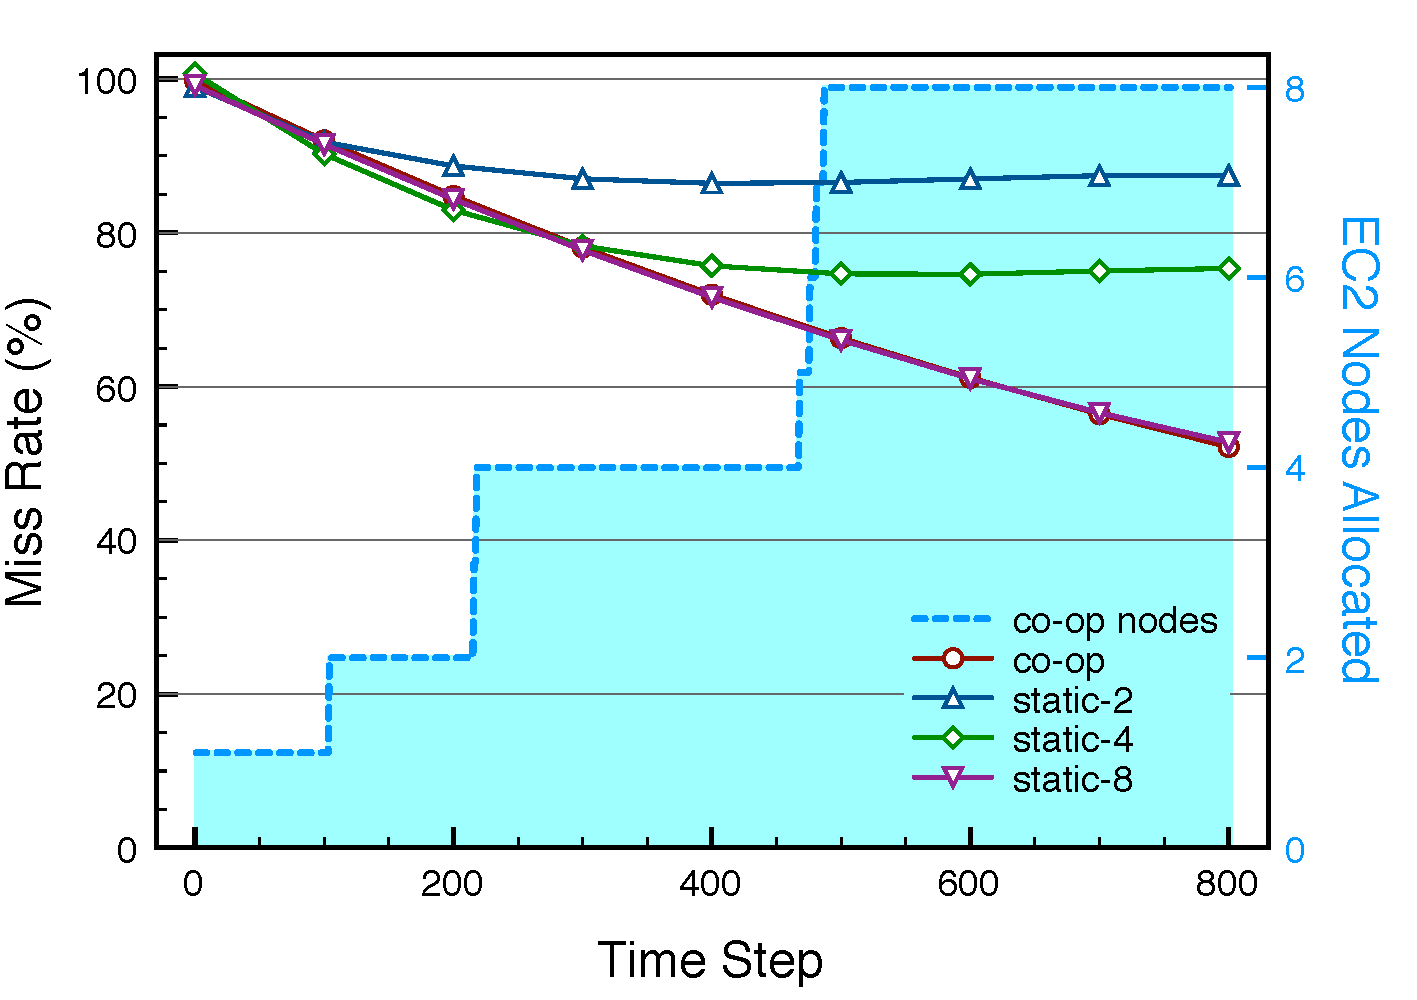
\includegraphics[scale=0.3]{figures/missrates_50.pdf}}
	\subfigure[Querying Rate = 255 queries/timestep]
	{\label{fig:rate-255-c}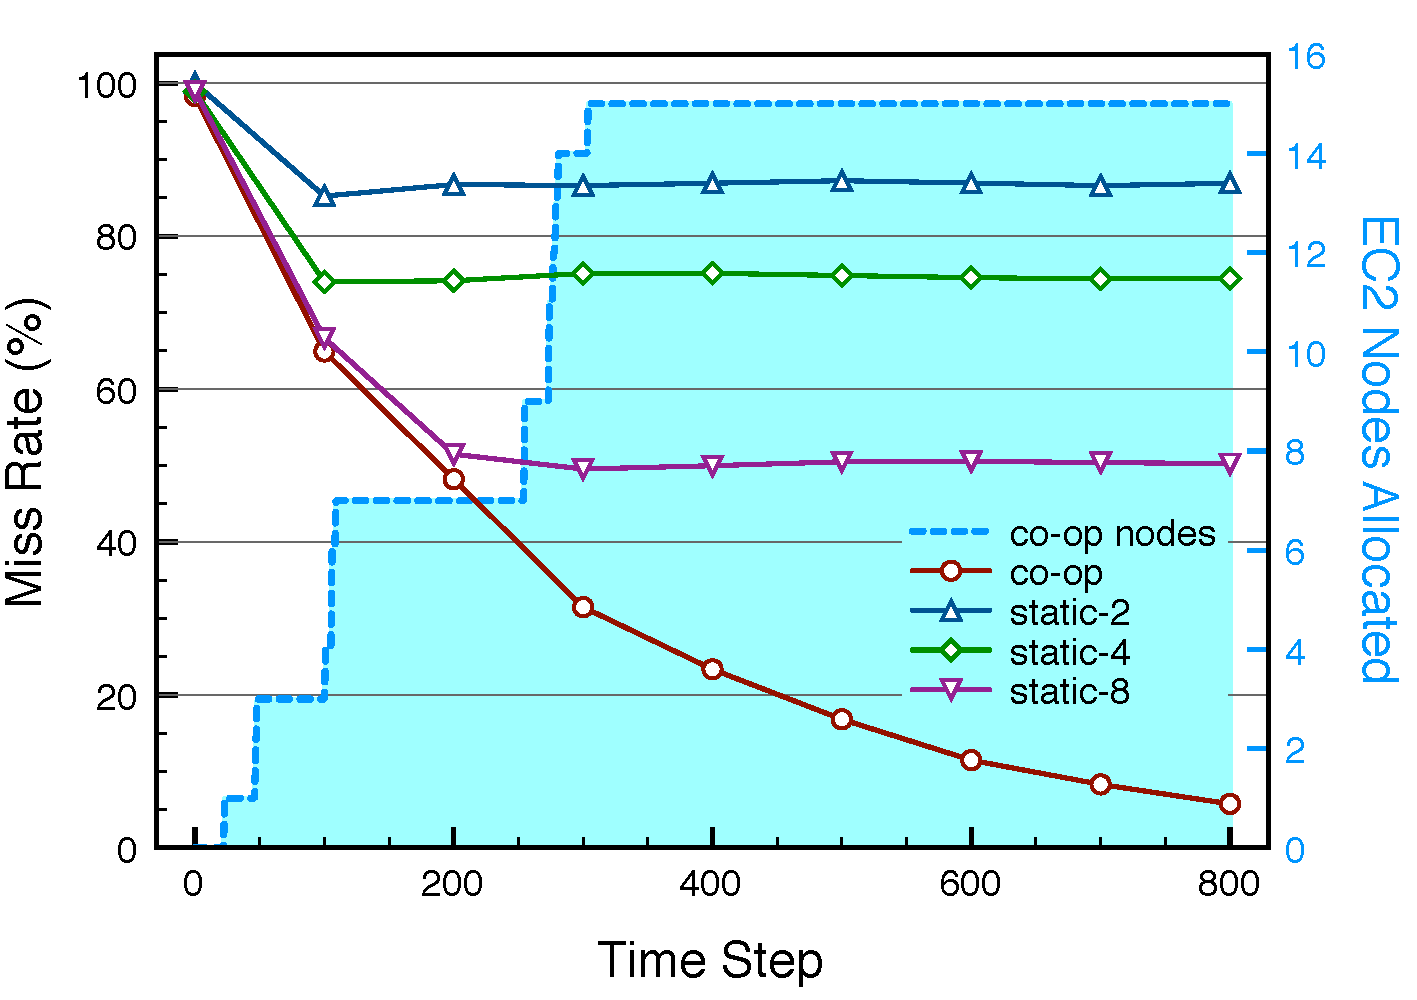
\includegraphics[scale=0.3]{figures/missrates_255.pdf}}
   	\caption{Miss Rate}
\end{center}
\end{figure}

Figure~\ref{fig:rate-50-c} and Figure~\ref{fig:rate-255-c} represent the
results for miss rates for experiments conducted with 50 and 255 queries/time
step respectively. The $X$-axis represents the time steps elapsed in our
experiment (recall that a time step is not real time, but simulated time in
which $R$ queries are sent). The right-hand $Y$-axis represents the EC2 nodes
allocated throughout the experiment.

As the experiment proceeds, the miss rates decrease linearly, since requests
are submitted at random. {\tt static-2} and {\tt static-4} appear to converge
very early in the experiments, while {\tt static-8} seems to perform as well as
our system in Figure~\ref{fig:rate-50-c}. This implies, and indeed is supported
by the results, that our system uses a maximum of 8 nodes at the end of the
execution.

One aspect not shown here is the amount of time taken to split and migrate data
when a new node is allocated. This may be an expensive overhead that varies
depending on the index that is being used. We show an evaluation of the impact
of indexing schemes and their migration overheads next.

% subsection evaluation_elastic_static (end)

\subsection{Cache Server Index Comparison} % (fold)
\label{sub:index_comparison}
Here we compare the three indexing schemes, \bptrees ({\tt B+Tree}), Counting
Bloom Filter ({\tt CBF}), and Extendible Hashing with three bucket size
configurations ({\tt EH100}, {\tt EH300}, {\tt EH500}). We evaluate the
suitability of these algorithms based on the total time taken to run the
experiment, the total time taken to migrate records, and minimum, maximum, and
average time taken per migration. In these experiments, we are showing the
total time taken to interact with two querying models: 50 queries/time step and
255 queries/time step \emph{without} speculative migration. We will show the
optimization observed with speculative execution in a later subsection.

\begin{figure}[htp]
\begin{center}
\subfigure[Query rate = 50 Queries/timestep]{\label{fig:tt50}
  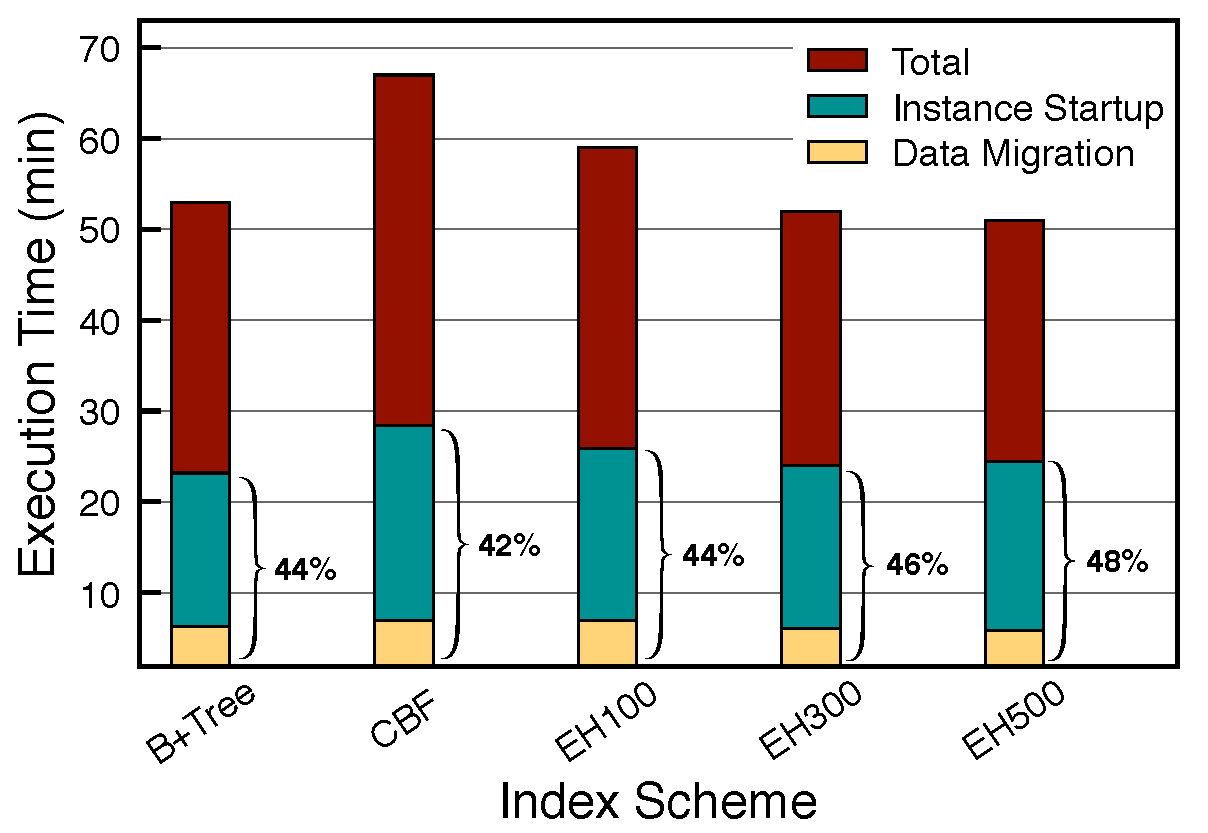
\includegraphics[scale=0.35]{figures/tt-50.pdf}}
\subfigure[Query rate = 255 Queries/timestep]{\label{fig:tt255}
  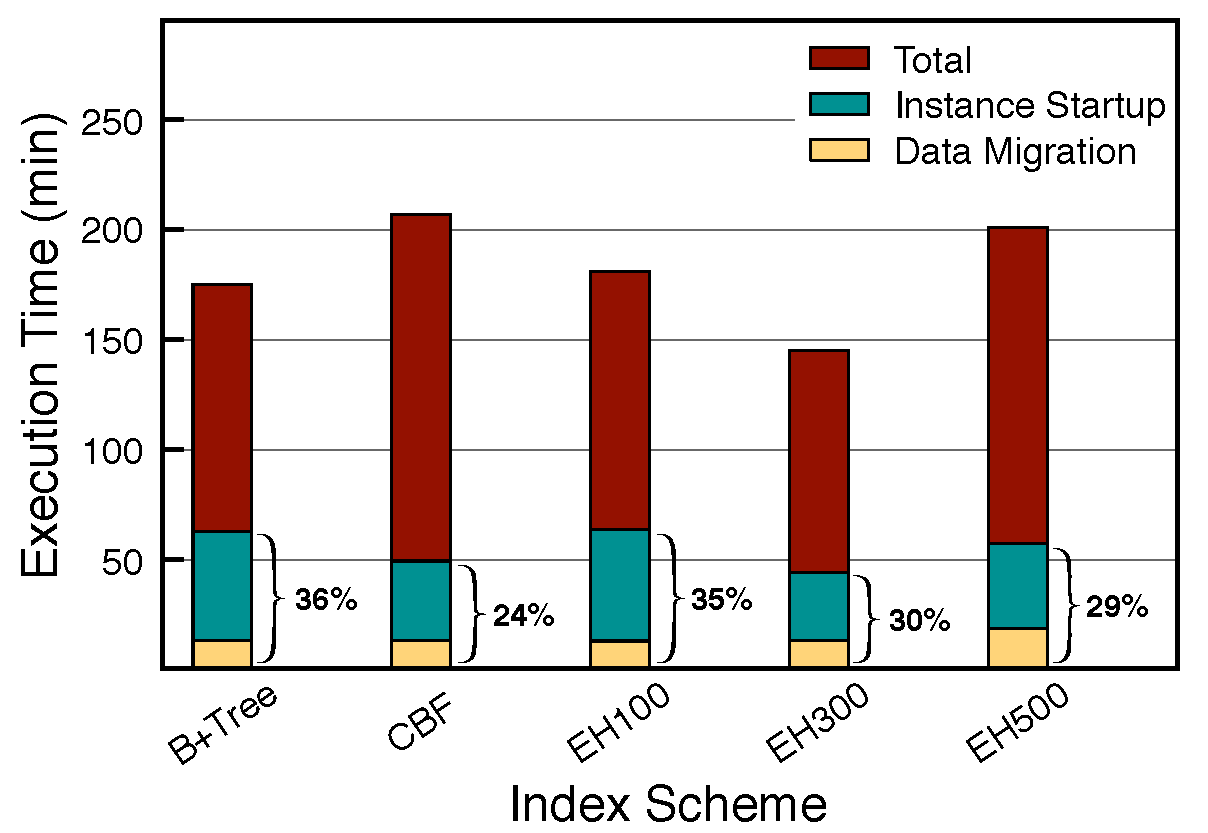
\includegraphics[scale=0.35]{figures/tt-225.pdf}}
\end{center}
\caption{Execution Time of Indexing Schemes}
\end{figure}

Figure~\ref{fig:tt50} shows the results obtained by running the experiment with
50 queries/time step, while Figure~\ref{fig:tt255} shows the results for 255
queries/time step. The total time taken to run the experiments varied between
50 and 70 minutes. As mentioned earlier, we note that instance startup times
can vary quiet heavily, and combined with data migration, the overhead accounts
for nearly half of the total execution time at 50 queries/time step. As
expected, the migration time for {\tt CBF} performs the worst, but is still
dominated by instance startup overhead. Although these overheads are amortized
as we increase the request rate to 255 queries/time step, they are still
significant.

In Figure~\ref{fig:tt50}, we can see that {\tt EH500} outperforms the rest,
while {\tt CBF} is clearly the worst option. We also can see that the system
parameter (records per bucket) has a great impact on the performance of
Extendible Hashing. The \bptree performs well regardless of parameters. This is
also reflected in Figure~\ref{fig:tt255} where {\tt EH300} performs the best
and {\tt CBF} once again performs the worst. Notably, the performance of {\tt
EH500} records per bucket has degraded quite considerably, while the
performance of the \bptree scales quite well even when the query intensity is
increased. Thus, we propose that the performance of Extendible Hashing also
depends upon the querying rate.

\begin{figure}[htp]
\begin{center}
\subfigure[Query rate = 50
  Queries/timestep, $7 \times$
  Migration]{\label{fig:mig50}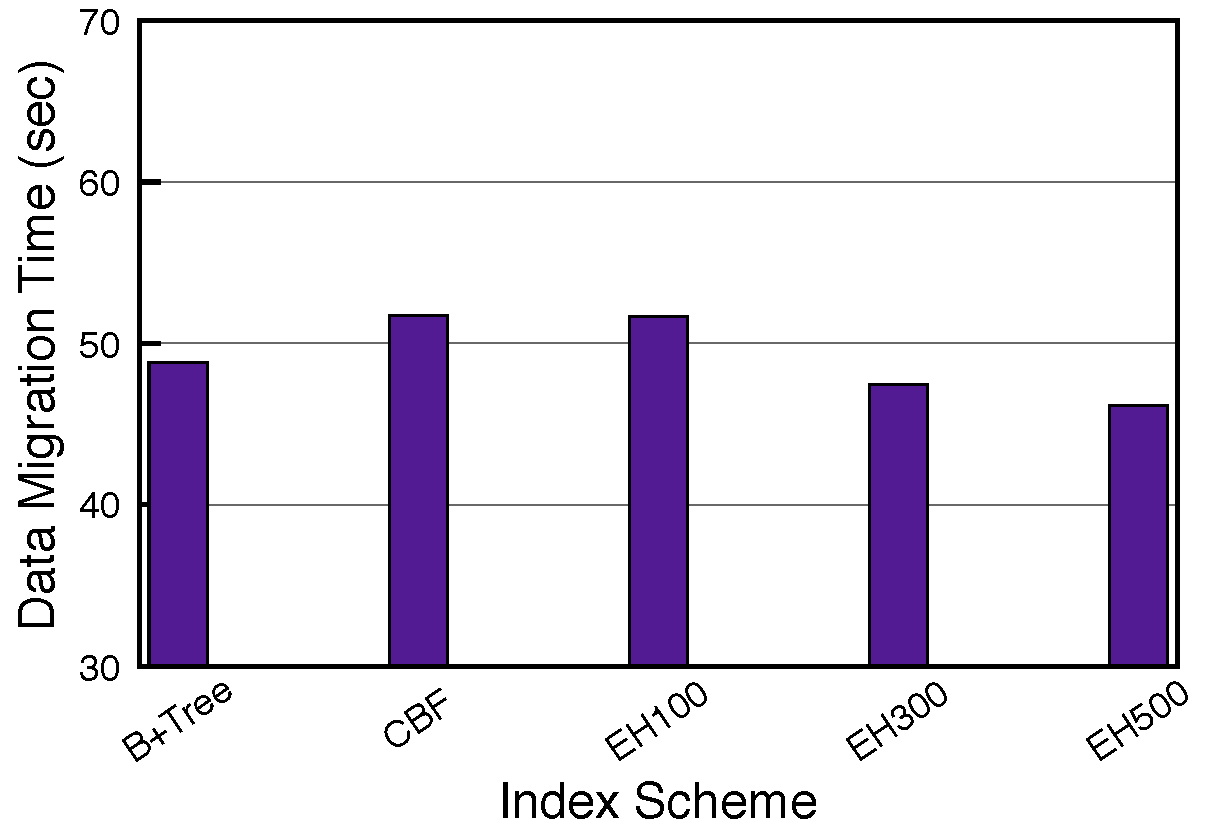
\includegraphics[scale=0.35]{figures/mig-50q.pdf}}
\subfigure[Query rate = 255
  Queries/timestep, $15 \times$
  Migration]{\label{fig:mig255}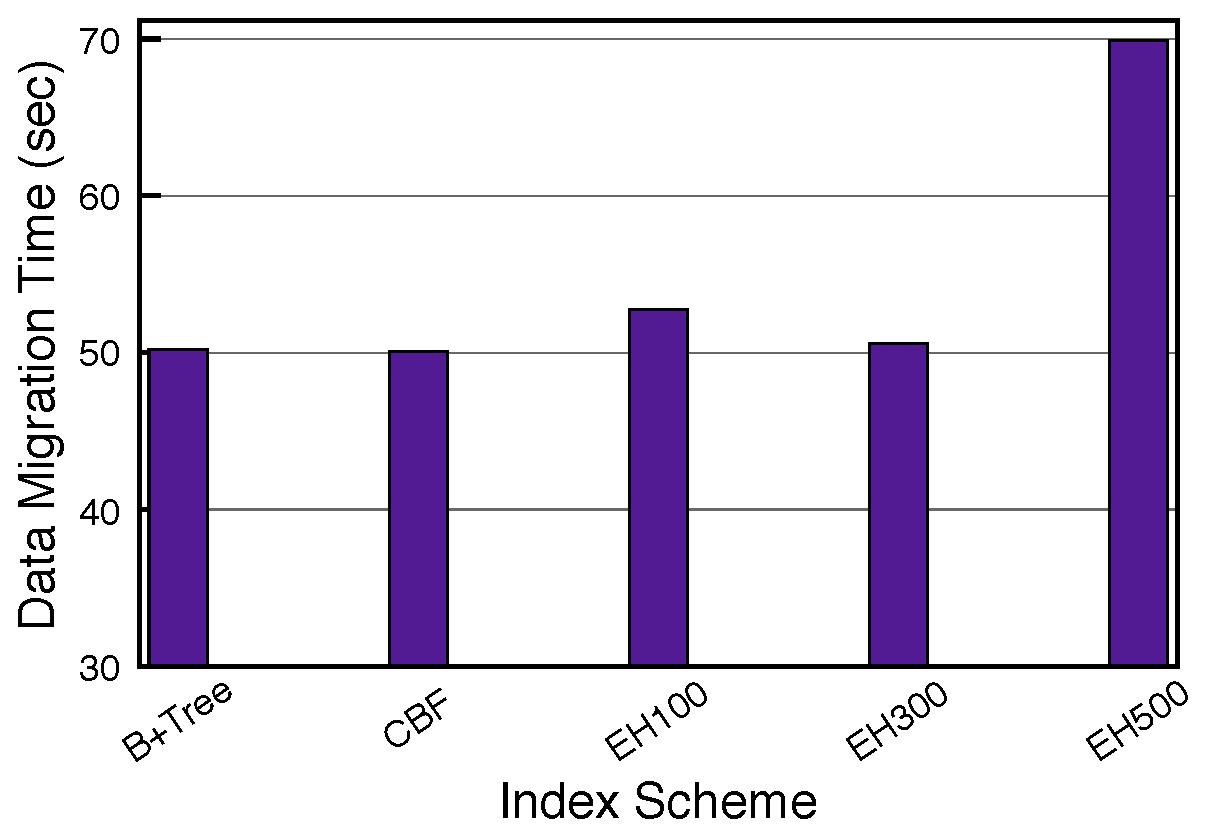
\includegraphics[scale=0.35]{figures/mig-225q.pdf}}
\end{center}
\caption{Migration Time of Indexing Schemes}
\end{figure}

In Figures~\ref{fig:mig50} and~\ref{fig:mig255}, we have averaged the time
taken per data migration, that is, the time taken to identify the range of data
to be transferred from the overflown node to the new node and the transferral
of that data. In total, migrations were invoked 7 times for 50 queries/time
step and 15 times for 255 queries/time step. We observe that there is not much
variation between the two graphs for \bptrees, suggesting that it scales well
to high request rates.

Interestingly, on average, {\tt CBF} performs better as the number of
migrations increases. This is due to the fact that the number of records to
be migrated decreases over time across all indexing schemes as a result of the
consistent hashing scheme. Over time, the ranges on the consistent hashing ring
will decrease. As we recall from Section~\ref{sec:bloom_filters}, migration on
{\tt CBF} is slightly super-linear due to the scan for false-positives. As the
data range decreases over time, false-positives also decrease, and the
algorithm comes closer to linear time. As we see in Figure~\ref{fig:mig255},
{\tt CBF} is eventually equivalent to B$^+$-Tree's linear-time migrations.

We can apply the same logic to explain the degradation in performance for the
{\tt EH*} schemes, all of which perform worse as the number of migrations
increase. Using the worst case, {\tt EH500} as an example, the average
migration times are quite low when we have fewer migrations because there are a
smaller number of buckets to traverse linearly. As the number of migrations
increase, this would imply that a greater quantity of data is being stored in
the index, which translates not only to a larger directory size (which grows
exponentially), but potentially many more buckets with data in the range
scattered amongst it. In other words, we observe the inherent problem of
hashing-based solutions for handling ranges. The tradeoff is that the $O(1)$
lookup facilitates fast hit/miss indication, leading to a better overall
performance for high querying rates.

To summarize, we observe that \bptrees scale well regardless of system
parameters, and Extendible Hashing, with its constant-time exact-match
searches, could outperform \bptrees if their parameters are chosen
appropriately. However, if the cache system is volatile and migration is
invoked often, Extendible Hashing indexing schemes will result in increasingly
poor migration performance. We also note that Counting Bloom Filters should
generally be avoided as an indexing scheme for elastic key-value storage. As a
caveat, however, CBF may scale well for applications relying on space-efficient
structures. We also make note of the interesting observation that CBF migration
overheads become better over time.

% subsection index_comparison (end)

\subsection{Indexing Optimization} % (fold)
\label{sub:indexing_optimization}
In Section~\ref{sec:elastic_cache_support} we described an approach for
minimizing idle-times when migrating data to newly allocated EC2 nodes.
Instances are pre-launched when some threshold is met and the migration
occurs in parallel to normal program execution. The results have been
summarized in Figure~\ref{fig:opt_prelaunch}. On the left side, we show the original
results for {\tt EH300} and {\tt CBF}. The right side depicts the results after
applying speculative prelaunching.

\begin{figure}[htp]
\centering
 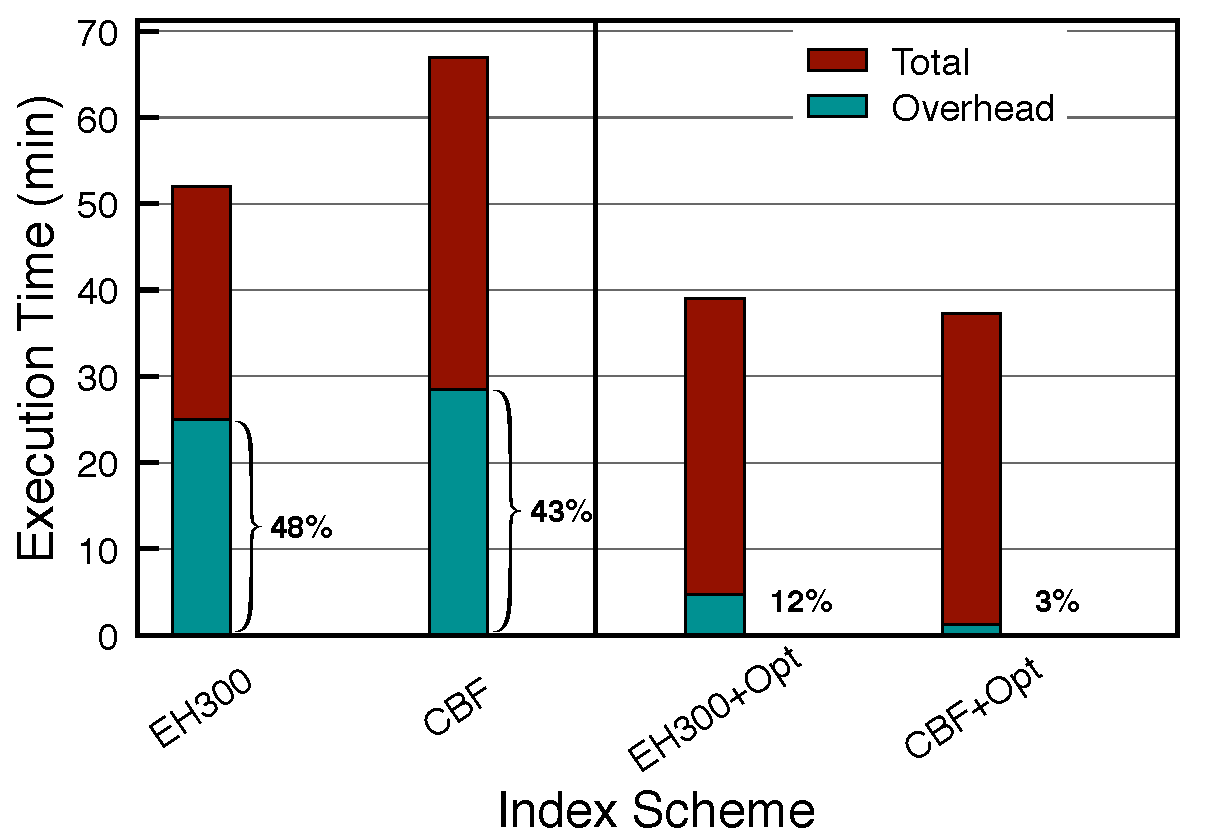
\includegraphics[scale=0.35]{figures/overhead-50.pdf} \\
\caption{\label{fig:opt_prelaunch}Optimization Results for Query Rate = 50
queries/timestep.}
\end{figure}

We executed a total of three runs and reported the average overhead and total
times. After optimization, we managed to improve overhead by $4\times$ and
$14\times$  in {\tt EH300} and {\tt CBF} respectively. Even with the
improvements, there are clear opportunities for further refinement and we
propose developing more robust heuristics in future works.

% subsection indexing_optimization (end)

\subsection{Performance-Cost Analysis} % (fold)
\label{sub:performance_cost_analysis}

% TODO: Rewrite this properly instead of C&Ping IJNGC...

To analyze the performance and cost tradeoffs, we use only the B$^+$-Tree
version and we run experiments over the following configurations:
\begin{enumerate}
\item {\tt S3}: Data stored as files directly onto the S3
storage service (persistent).
\item {\tt ec2-m1.small-mem}: Data stored in memory on Small EC2 instance
(volatile, moderate I/O).
\item {\tt ec2-m1.small-disk}: Data stored as files on disk on Small EC2
instance (volatile, moderate I/O).
\item {\tt ec2-m1.small-ebs}: Data stored as files on a mounted Elastic Block
Store volume on small EC2 instance (persistent, moderate I/O).
\item {\tt ec2-m1.xlarge-mem}: Data stored in memory on Extra Large EC2 instance
(volatile, high I/O). 
\item {\tt ec2-m1.xlarge-disk}: Data stored as files on disk on Extra Large EC2
instance (volatile, high I/O).
\item {\tt ec2-m1.xlarge-ebs}: Data stored as files on a mounted Elastic Block
Store volume on Extra Large EC2 instance (persistent, high I/O).
\end{enumerate}

Within the EC2 instances, we evaluate three disparate ways to store the cache:
in-core ({\tt *-mem}), on local disk ({\tt *-disk}), and on Amazon's Elastic
Block Storage, or simply EBS ({\tt *-ebs}). In both {\tt m1.small} (32-bit)
and {\tt m1.xlarge} (64-bit) systems, we employ the Ubuntu Linux 9.10 Server
image provided by Alestic.\footnote{Alestic, http://alestic.com/}

To analyze cache and storage performance, which can be affected by
memory size, disk speed, network bandwidth, etc., we varied the
sizes of cached files: $1$ KB, $1$ MB, $5$ MB, $50$ MB\@. One such file is output
from one execution, and over time, we would need to store a series of such
files in our cache. These sizes allow for scenarios from cases where all cached
data can fit into memory (e.g., $1$ KB, $1$ MB) to cases where in-core
containment would be infeasible (e.g., $50$ MB), coercing the need for disk or
S3 storage. The larger data will also amortize network latency and
overheads, which increases throughput. 

We submitted queries to hot caches, which guarantees a hit on every query, and
we are reporting the mean time in seconds to search the cache and retrieve the
relevant file \textit{on one cache node}.
Figures~\ref{fig:1kb-exectime},~\ref{fig:1mb-exectime},~\ref{fig:5mb-exectime},
and~\ref{fig:50mb-exectime} show the average \textit{hit} times for each cache
configuration. 
\begin{figure}
\begin{center}
	\subfigure[Data Size = 1 KB]
	{\label{fig:1kb-exectime}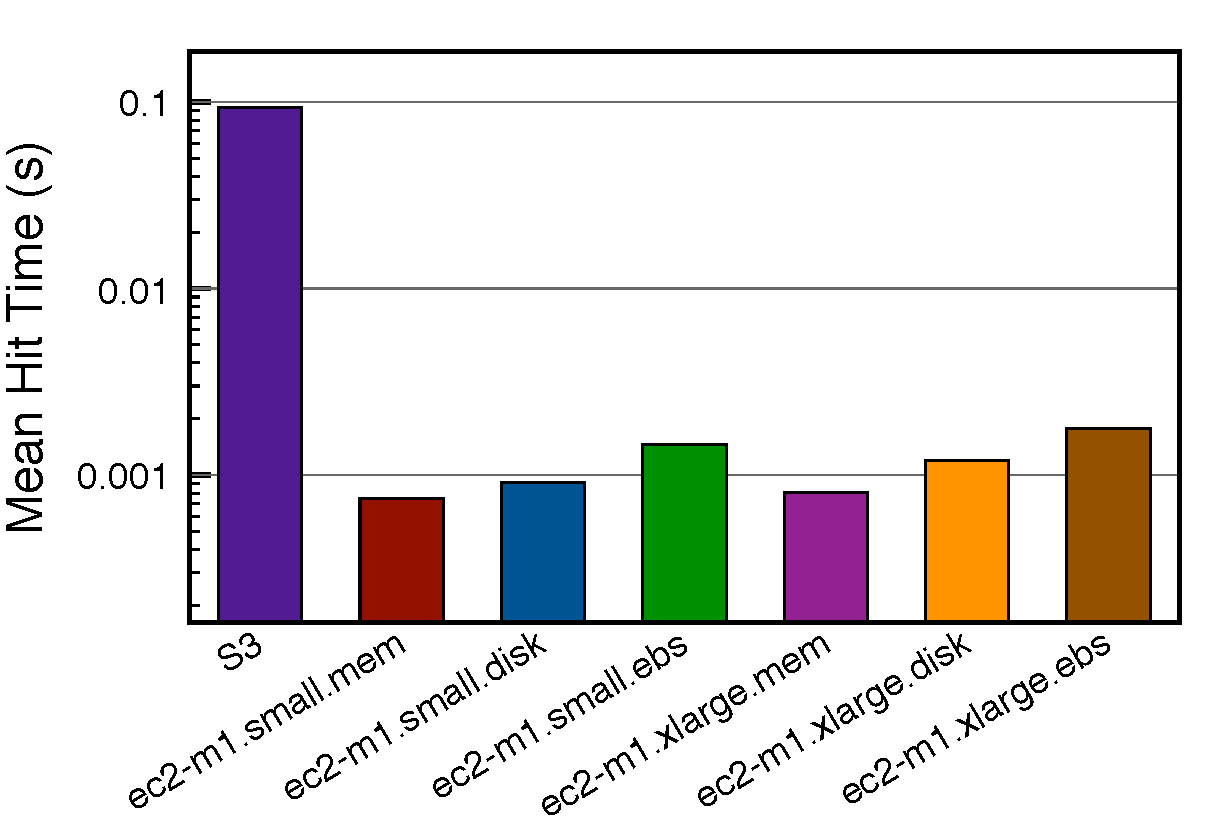
\includegraphics[scale=0.35]{figures/1kb-hitspeedup.pdf}}
	\subfigure[Data Size = 1 MB]
	{\label{fig:1mb-exectime}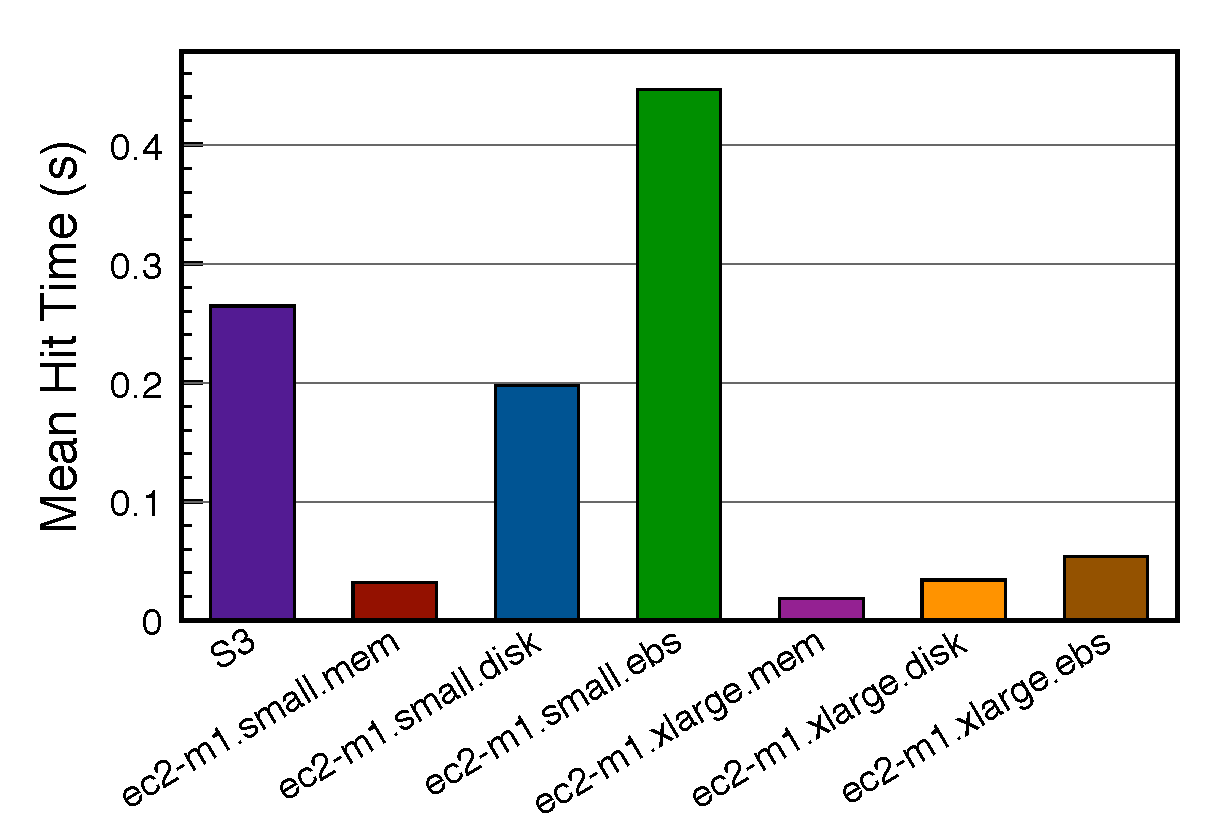
\includegraphics[scale=0.35]{figures/1mb-hitspeedup.pdf}}
  \\
	\subfigure[Data Size = 5 MB]
	{\label{fig:5mb-exectime}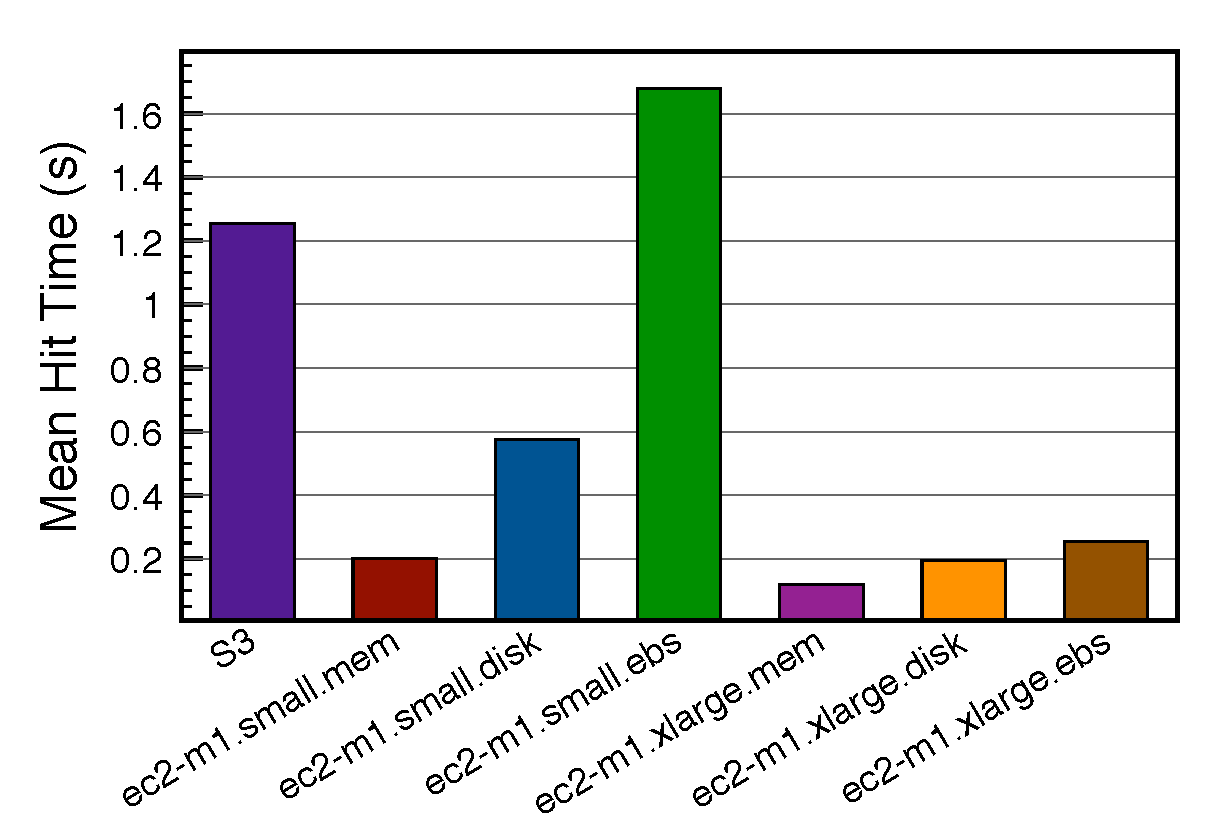
\includegraphics[scale=0.35]{figures/5mb-hitspeedup.pdf}}
	\subfigure[Data Size = 50 MB]
	{\label{fig:50mb-exectime}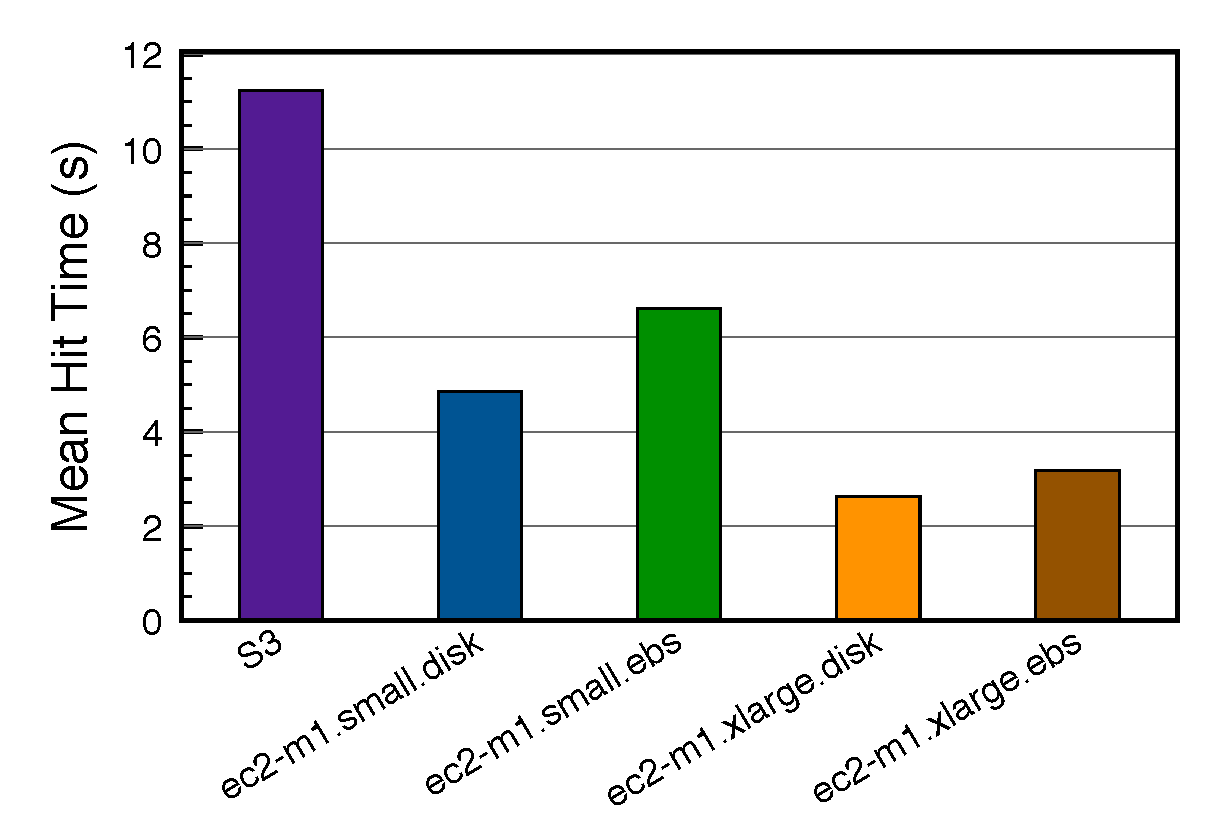
\includegraphics[scale=0.35]{figures/50mb-hitspeedup.pdf}}
	\caption{\label{fig:Speedup}Mean Cache Hit + Retrieval Time}
\end{center}
\end{figure}

Figure~\ref{fig:1kb-exectime} shows that using {\tt S3} for small files
eventually exhibits slowdowns by $2$ orders of magnitude. In the other figures,
we observe the justification for using memory-bound configurations, as they
exhibit for the lowest mean hit times. Also, we observe consistent slowdowns
for {\tt ec2-m1.small-disk} and {\tt ec2-m1.small-ebs} below {\tt S3} in the 1
MB and 5 MB cases.  Finally, using the results from
Figure~\ref{fig:50mb-exectime}, we can conclude that these results again
support our belief that disk-bound configurations of the small instance types
should be avoided for such mid-sized data files due to disk access latency.
Similarly for larger files, {\tt S3} should be avoided in favor of {\tt
ec2-m1.xlarge-ebs} if persistence is desirable. We have also ascertained from
these experiments that the \textit{high} I/O that is promised by the extra
large instances contributes significantly to the performance of our cache.

\begin{sidewaystable}[htp]
\small
\caption{Monthly Cache Subsistence Costs: Volatile (Top), Persistent (Bottom)}
\label{tab:systemcosts}
\begin{minipage}{5cm}
\begin{tabular}{|c|l|l|l|l|||l|l|l|}
\hline
& & \multicolumn{3}{c|||}{2000 Requests} & \multicolumn{3}{c|}{200000 Requests} \\
\hline
\textbf{Unit-Size} & & $S$ & \textbf{$C = C_{Alloc} + C_{IO}$} & $C/S$ & $S$ & $C_{IO}$ & ${C/S}$\\
\hline
{$1$ KB} & {\tt m1.small-mem} & $3.54$ & $\$63.24 = \$63.24 + \$0.00$ & $\$17.84$ & $2629.52$ & $\$0.03$ & $\$0.03$\\ (500 KB total) & {\tt m1.small-disk} & $3.67$ & $\$63.24 + \$0.00 = \$63.24$ & $\$17.23$ & $2147.681$ & $\$0.03$ &  $\$0.03$\\
& {\tt m1.xlarge-mem} & $3.64$ & $\$505.92 = \$505.92 + \$0.00$ & $\$138.99$  & $2302.43$ & $\$0.03$ & $\$0.22$\\
& {\tt m1.xlarge-disk} & $3.63$ & $\$505.92 = \$505.92 + \$0.00$& $\$139.57$  & $1823.215$ & $\$0.03$ & $\$0.28$\\
\hline
{$1$ MB} & {\tt m1.small-mem} & $3.5$ & $\$63.54 = \$63.24 + \$0.30$ & $\$18.17$ & $267.19$ & $\$30.00$ & $\$0.35$\\
(500 MB total) & {\tt m1.small-disk} & $3.26$ & $\$63.54 = \$63.24 + \$0.30$ & $\$19.49$ & $28$ & $\$30.00$ & $\$4.06$\\
& {\tt m1.xlarge-mem} & $3.6$ & $\$506.22 = \$505.92 + \$0.30$ & $\$140.62$ & $347.3$ & $\$30.00$& $\$1.53$\\ & {\tt m1.xlarge-disk} & $3.59$ & $\$505.92 + \$0.30 = \$506.22$ & $\$141.13$ & $180.53$ &  $\$30.00$ &$\$2.94$\\
\hline
{$5$ MB} & {\tt m1.small-mem} & $3.3$ & $\$444.18 = \$442.68 + \$1.50$ & $\$96.27$ & $109.47$ & $\$150.00$ &$\$4.26$\\
(2.5 GB total) & {\tt m1.small-disk}& $3.2$ & $\$64.74 = \$63.24 + \$1.50$ & $\$20.24$ & $33.84$ & $\$150.00$ &$\$6.30$\\
& {\tt m1.xlarge-mem} & $3.6$ & $\$506.78 = \$505.92 + \$1.50$ & $\$140.78$ & $174.42$ & $\$150.00$ & $\$3.76$\\
& {\tt m1.xlarge-disk} & $3.38$ & $\$506.78 = \$505.92 + \$1.50$ & $\$149.94$ & $111.71$ & $\$150.00$ & $\$5.87$\\
\hline
{$50$ MB}
& {\tt m1.small-disk} & $2.9$ & $\$78.74 = \$63.24 + \$15.00$ & $\$27.16$ & $16.05$ & $\$1500.00$ & $\$97.40$\\
(25 GB total) & {\tt m1.xlarge-disk} & $3.31$ & $\$520.92 = \$505.92 + \$15.00$ & $\$152.85$ & $31.66$ & $\$1500.00$ &$\$63.36$\\
\hline
\end{tabular}
\end{minipage}
\vspace{0.5cm}

\begin{minipage}{5cm}
\begin{tabular}{|c|l|l|p{6.2cm}|l|||l|l|l|}
\hline
& & \multicolumn{3}{c|||}{2000 Requests} & \multicolumn{3}{c|}{200000 Requests} \\
\hline
\textbf{Unit-Size} & & $S$ & \textbf{$C_{S3} = C_S + C_{R} + C_{IO}$ \newline $C_{EBS} = C_{Alloc} + C_{S} + C_{R} + C_{IO}$} & $C/S$ & $S$ & $C_{IO}$ & ${C/S}$\\
\hline
{$1$ KB} & {\tt S3} & $3.4$ &  $\$0.0023 = \$0.00 + \$0.002 + \$0.0003$ & $\$0.0007$ & $24.79$ &  $\$0.23$ & $\$0.01$\\
(500 KB total)& {\tt m1.small-ebs} & $3.62$ & $\$63.49 = \$63.24 + \$0.0002 + \$0.00 + \$0.0003$ & $\$17.54$ & $1984.5$ & $\$0.48$ & $\$0.04$\\
& {\tt m1.xlarge-ebs} & $3.58$ & $\$506.17 = \$505.92 + \$0.0002 + \$0.00 + \$0.0003$ & $\$141.39$ & $2091.7$ & $\$0.48 $ &$\$0.25$\\
\hline
{$1$ MB} & {\tt S3} & $3.39$ & $\$0.38 = \$0.075 + \$0.002 + \$0.30 $ & $\$0.12$ & $29.98$ & $\$30.01$ & $\$1.01$\\
(500 MB total)& {\tt m1.small-ebs} & $2.95$ & $\$63.59 = \$63.24 + \$0.05 + \$0.00 + \$0.30$ & $\$21.56$ & $13.62$ &  $\$30.25$ & $\$6.87$\\
& {\tt m1.xlarge-ebs} & $3.57$ & $\$506.27 = \$505.92 + \$0.05 + \$0.00 + \$0.30$ & $\$142.00$ & $133.96$ &  $\$30.25$ &$\$4.01$\\
\hline
{$5$ MB} & {\tt S3} & $3.27$ &  $\$1.88 = \$0.375 + \$0.002 + \$1.50$ & $\$0.58$ & $19.97$ & $\$150.00$ & \$7.53\\
(2.5 GB total)& {\tt m1.small-ebs} & $2.83$ & $\$64.99 = \$63.24 + \$0.25 + \$0.00 + \$1.50$ & $\$22.97$ & $11.84$ & $\$150.27$ & $\$18.04$\\
& {\tt m1.xlarge-ebs} & $3.3$ &  $\$507.67 = \$505.92 + \$0.25 + \$0.00 + \$1.50$ & $\$153.92$ & $74.66$ & $\$150.27$ &$\$8.79$\\
\hline
{$50$ MB} & {\tt S3} & $2.59$ & $\$18.75 = \$3.75 + \$0.002 + \$15.00$ & \$7.24 & $6.43$ &  $\$1500.00$ & $\$233.87$\\
(25 GB total)& {\tt m1.small-ebs} & $2.74$ & $\$80.74 = \$63.24 + \$2.50 + \$0.00 + \$15.00$ & $\$29.47$ & $11.09$ &  $\$1502.52$ & $\$142.70$\\
& {\tt m1.xlarge-ebs} & $3.16$ & $\$520.42 = \$505.92 + \$2.50 + \$0.00 + \$15.00$ & $\$164.69$ & $22.66$ & $\$1502.52$ & $\$88.63$\\
\hline
\end{tabular}
\end{minipage}
\end{sidewaystable}

We now present an analysis on cost for the instance configurations being
considered. The costs of the AWS features evaluated in our experiments are
summarized in Table~\ref{tab:systemcosts}. While in-Cloud network I/O is
currently free, in practice, we cannot assume that all users will be able to
compute within the same Cloud.  We thus assume that cache data is transferred
outside of the AWS Cloud network in our analysis.

We are repeating the settings from the previous set of experiments, so an
average unit data size of $50$ MB will yield a total cache size of $25$ GB of
Cloud storage (assuming there are $500$ distinct request keys). We are
furthermore assuming a fixed rate of $R = 2000$ requests per month from clients
outside the Cloud. We have also extrapolated the costs (right side of table)
for when request rate $R = 200000$, using the Mean Hit Times from
Figure~\ref{fig:Speedup} as the limits for such a large request rate $R$.
Clearly, as $R$ increases for a full cache, the speedup given by cache will
eventually become denominated by the Mean Hit Times.

For these experiments, we start with a cold cache.  The cost, $C$, of
maintaining the cache, the average speedup $S$ per request (after $2000$ and
$200000$ requests), and the ratio $C/S$ (i.e., the cost per unit-speedup), are
reported under two requirements: volatile and persistent data stores. Again,
volatile caches are less reliable in that, upon a node failure, all data is
lost. The costs for sustaining a volatile cache for one month is reported in
Table~\ref{tab:systemcosts} (top).  Here, the total cost can be computed as $C
= (C_{Alloc} + C_{IO})$, where $C_{Alloc} = h \times k \times c_t$ denotes
hours, $h$ to allocate some $k$ number of nodes using the said costs (from
Table~\ref{tab:systemcosts}) for instance type $t$. $C_{IO} = R \times d \times
c_{io}$ accounts for transfer costs, where $R$ transfers were made per month,
each involving $d$ GB of data per transfer, multiplied by the cost to transfer
per GB, $c_{io}$.

First, we recall that if the unit-data size, $d$, is very small ($1$ KB), we can
obtain excellent performance for any volatile configuration. This is because
everything easily fits in memory, and we speculate that, even for the
disk-based options, the virtual instance is performing its own
memory-based caching, which explains why performance is not lost. This is
further supported by the speedup when $d = 1$ MB, under the disk-based option.
When projected to $R = 200000$ requests, we observe lucrative speedups, which
is not surprising, considering the fast access and retrieval times for such a
small file. Furthermore, when $R = 2000$ requests, the {\tt ec-m1.small-disk} 
option offers excellent $C/S$ ratios, making it a very good option.
Conversely, when request rate $R$ is large, the I/O performance of the small
instances accounts for too much of a slowdown, resulting in low speedups, and
a low $C/S$ ratio. This suggests that {\tt m1.xlarge} is a better option for
systems expecting higher throughput rates.

Next, we compiled the cost for persistent caches, supported by {\tt S3} and
{\tt EBS} in Table~\ref{tab:systemcosts} (bottom). Here, $C_S$ refers to the
cost per $1$ GB-month storage, $C_{R}$ is the request cost, and $C_{IO}$ refers
to the data transfer costs per GB transferred out.  Initially, we were
surprised to see that {\tt S3}'s $C/S$ ratio is comparable to {\tt EBS} (and
even to the volatile options) when request rate $R$ is low regardless of data
size. However, for a large request rate, $R$, its overhead begins to slowdown
its performance significantly compared to {\tt EBS} options.  Especially
observed when unit-size, $d$, is very small, {\tt S3}'s speedup simply pales in
comparison to other options. Its performance expectedly increases as $d$
becomes larger, due to the amortization of overheads when moving larger files.
This performance gain of {\tt S3}, however, drops sharply when $d = 50$ MB,
resulting in only $6.43\times$ speedup, making {\tt EBS} better options in
terms of cost per unit-speedup.

% subsection performance_cost_analysis (end)

\subsection{Hybrid Cache Evaluation} % (fold)
\label{sub:hybrid_system_evaluation}
We built the hybrid cache mentioned in Section~\ref{sec:hybrid_system} and ran
the following experiments on one {\tt m1.xlarge} node. Using 5 MB unit size, we
randomly submitted 3000 unique keys over 5000 requests. We also submitted 1000
requests over 500 unique keys for 25 MB unit size. We measured their miss
rates, as shown in Figures~\ref{fig:5mb-S3evict} and~\ref{fig:25mb-S3evict}
respectively. The subgraphs within each figure show the number of records that
have been evicted into S3. As can be seen in both figures, the hybrid cache
offers lower miss rates, which results in lower average request times. This
pattern is more prominent and occurs sooner in Figure~\ref{fig:25mb-S3evict}
due to a lower key range being used in the experiment. We do not offer the
same, in-depth cost analysis as in section~\ref{sub:performance_cost_analysis}.

\begin{figure}[htp]
\begin{center}
	\subfigure[Data Size = 5 MB]
	{\label{fig:5mb-S3evict}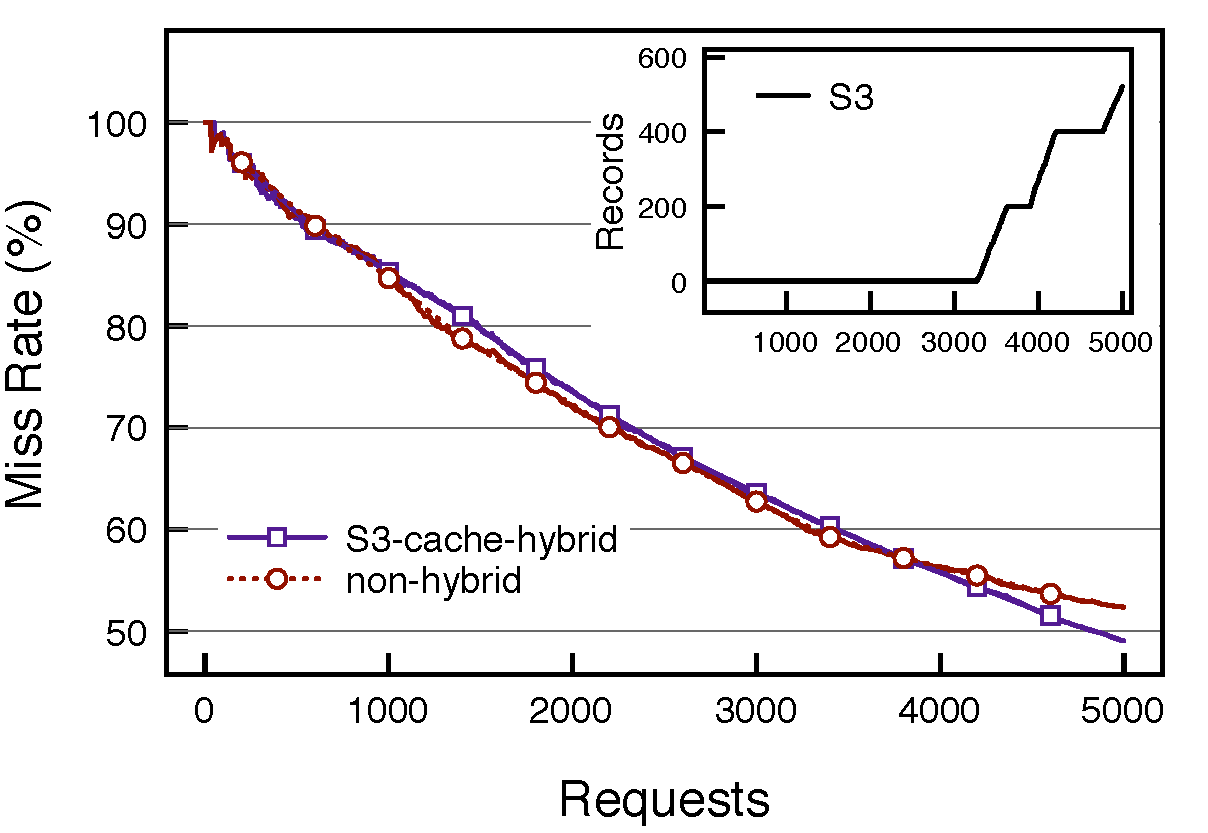
\includegraphics[scale=0.35]{figures/s3evict-05.pdf}}
	\subfigure[Data Size = 25 MB]
	{\label{fig:25mb-S3evict}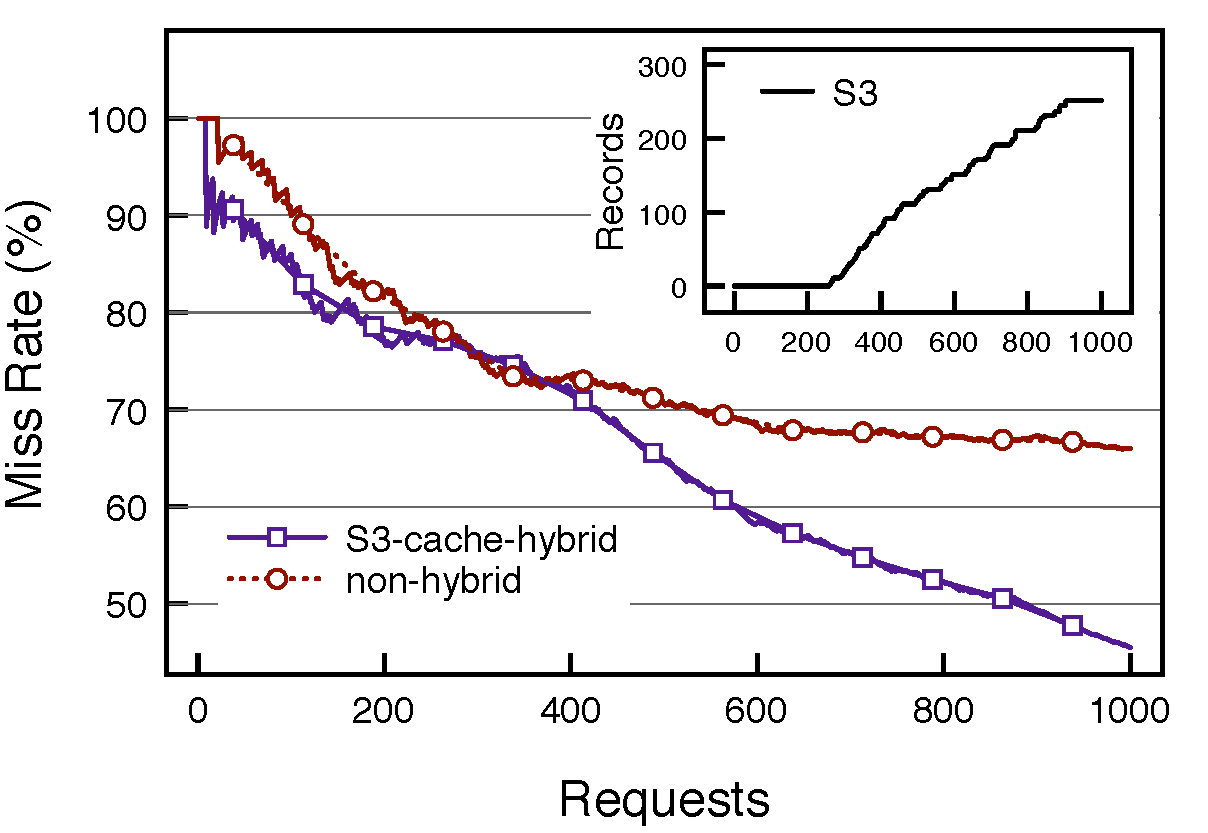
\includegraphics[scale=0.35]{figures/s3evict-25.pdf}}
	\caption{Miss Rates for S3-Eviction Hybrid Cache}
\end{center}
\end{figure}

% subsection hybrid_system_evaluation (end)

% section results_indexing (end)
